\documentclass[letterpaper]{article}
\usepackage{aaai2027}
\usepackage{times}
\usepackage{helvet}
\usepackage{courier}
\usepackage[hyphens]{url}
\usepackage{graphicx}
\urlstyle{rm}
\def\UrlFont{\rm}
\usepackage{natbib}
\usepackage{caption}
\frenchspacing
\setlength{\pdfpagewidth}{8.5in}
\setlength{\pdfpageheight}{11in}

\title{Leaderless Semantic Allocation: Measuring What Consensus Auctions Buy LLM-Driven Robot Teams Under Communication Degradation and Agent Churn}
\author{
    Dominic Dawes\textsuperscript{\rm 1}
}
\affiliations{
    \textsuperscript{\rm 1}University of Maryland, Baltimore County\\
    1000 Hilltop Circle, Baltimore, Maryland 21250\\
    ddawes2@umbc.edu
}

\begin{document}
\maketitle
\begin{abstract}
As robot teams adopt large language and vision-language models (LLMs/VLMs) as per-agent reasoners, coordination is expected to hold outside controlled facilities, where communication links are range-limited or degraded and agents drop out of and rejoin the team mid-mission. Current LLM-driven multi-robot systems coordinate through a centralized orchestrator or through natural-language negotiation between agents, and are evaluated almost exclusively under perfect communication. Under packet loss or network partition, agents may claim the same task, abandon tasks held by a failed teammate, or act on a stale belief of what has been completed. None of these failures is detected before it reaches the environment.

Classical decentralized allocation algorithms, both consensus-based (CBBA) and market-based (MURDOCH, TraderBots), provide conflict-free assignment and degrade gracefully under changing network topology, but they score tasks with hand-specified numeric utilities that cannot represent constraints stated only in natural language. Recent decentralized LLM frameworks recover semantic reasoning but reintroduce elected leaders and do not isolate the effect of communication impairment. We ask whether grounding per-agent LLM reasoning in a consensus auction preserves coordination under degraded communication and agent churn, and what that added structure costs relative to unconstrained LLM coordination.

We propose a leaderless architecture in which each agent's LLM generates a bundle-independent utility $u_{ij}$ for each task $\tau_j$ from the task's natural-language description and the agent's capabilities. A consensus auction resolves the allocation, and each agent executes its bundle by tool-calling action primitives. Allocation and execution state are held in a replicated per-agent ledger with monotone task status and lease-based ownership, and each agent's action history is compacted after $N$ entries. We evaluate five coordination conditions: a centralized oracle with ground-truth feasibility, decentralized LLM-only negotiation, CBBA with numeric-only utilities, LLM+CBBA, and LLM+MURDOCH. Each condition is run under perfect communication and swept across packet loss rate $p$, communication range $r$, and $k$-agent dropout and rejoin, in a heterogeneous multi-robot task environment. We measure utility relative to the oracle, duplicate and orphaned task rates, recovery time after dropout, ledger divergence, and token and message cost.

We hypothesize the following. First, LLM-generated utilities close the gap to the oracle in proportion to the fraction of tasks carrying language-only constraints; where constraints are purely geometric, numeric CBBA matches LLM+CBBA at a fraction of the cost. Second, we expect robustness and reasoning to come apart: LLM-only teams degrade sharply as $p$ rises and $r$ shrinks, through duplicated and orphaned tasks, while auction-based teams degrade gracefully, so the robustness gain is attributable to consensus and the replicated ledger rather than to the LLM. Finally, we expect a connectivity threshold below which consensus fails to converge within the replanning horizon, and below which greedy LLM-only coordination outperforms the auction.
\end{abstract}

\section{Introduction}
...

\begin{figure*}[t]
  \centering
  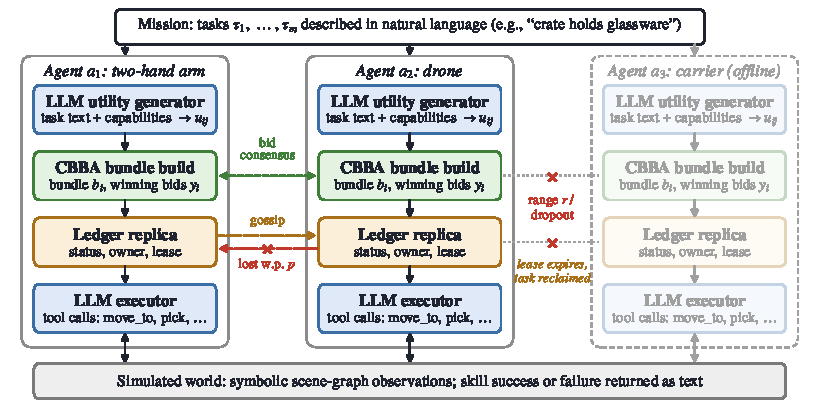
\includegraphics[width=\textwidth]{fig_architecture.pdf}
  \caption{Leaderless semantic allocation. Each agent's LLM converts natural-language task
  descriptions and its own capability card into bundle-independent utilities $u_{ij}$.
  CBBA builds a local bundle from these utilities, and agents reach a conflict-free
  assignment by exchanging bids with neighbors they can reach. Each agent keeps its own
  replica of the task ledger, synchronized by gossip over a lossy channel (messages lost
  with probability $p$). When an agent leaves communication range $r$ or drops out, its
  task leases expire and teammates reclaim the tasks. An LLM executor carries out each
  agent's bundle through tool calls to action primitives.}
  \label{fig:architecture}
\end{figure*}

\section{Related Work}
\label{sec:related}

We group prior work into five areas: classical decentralized task allocation, allocation under degraded communication, LLM-driven multi-robot coordination, task tracking and replicated state, and evaluation under communication impairment.

\subsection{Decentralized Task Allocation}

\paragraph{Contract Net.}
The Contract Net Protocol~\citep{smith1980contract} introduced announce--bid--award negotiation, in which a manager broadcasts a task and contractors bid to perform it. Every auction-based allocator we evaluate descends from this protocol. It assumes reliable messaging and numeric eligibility, whereas we evaluate bidding with LLM-derived utilities over a lossy channel.

\paragraph{Free-market architecture.}
\citet{dias2000free} proposed a market architecture in which robots trade tasks to maximize individual profit, which in aggregate lowers team cost. This work began the TraderBots line that our framing builds on. Its utilities are numeric revenue and cost functions and cannot express constraints stated only in natural language.

\paragraph{TraderBots.}
\citet{dias2004traderbots} developed the market approach into TraderBots, which aims for the solution quality of centralized planning with the robustness of distributed planning, including recovery from robot failure and communication loss. It addresses the same robustness question our churn sweep measures. We do not implement TraderBots as a condition for scope reasons, and our agents compute utilities with an LLM rather than engineered cost functions.

\paragraph{MURDOCH.}
MURDOCH~\citep{gerkey2002sold} allocates each task through a first-price single-item auction over a publish/subscribe network and reassigns tasks when a winner fails. It is our second auction family (LLM+MURDOCH), and its re-auction on failure parallels our dropout and rejoin condition. MURDOCH robots bid hand-coded fitness metrics, which we replace with per-agent LLM utilities.

\paragraph{CBBA.}
The Consensus-Based Bundle Algorithm~\citep{choi2009cbba} has each agent greedily build a bundle of tasks and then run consensus on the winning bids, so no auctioneer is needed. It guarantees a conflict-free assignment among connected agents and a bounded approximation when scores have diminishing marginal gains. CBBA is the allocation core of our main condition; we replace its numeric scores with bundle-independent LLM utility terms so that the diminishing-gains property is preserved.

\paragraph{Asynchronous CBBA.}
\citet{johnson2011acbba} removed CBBA's global synchronization so that agents converge using timestamped, asynchronous messages. This timestamp-based deconfliction is the closest classical precedent for our replicated ledger merge. ACBBA replicates allocation state only, while our ledger also replicates execution status, ownership leases, and action history.

\subsection{Allocation Under Degraded Communication}

\paragraph{Dynamic communication constraints.}
\citet{ponda2010dynamic} extended CBBA to heterogeneous teams with task time windows and communication links that change during the mission. It is a classical study of consensus allocation on a changing communication graph, which is our main experimental axis. It does not involve language-specified constraints, agent churn, or an execution ledger.

\paragraph{Auctions under limited communication.}
\citet{otte2020auctions} systematically compared auction variants under message loss and limited communication. It is the nearest classical analogue of our packet-loss sweep and informs our baselines and metrics. Its agents bid numeric costs, whereas we add LLM utilities, an LLM-only negotiation baseline, and agent dropout and rejoin.

\paragraph{Event-driven CBBA.}
\citet{sao2025edcbba} transmit CBBA messages only when an agent's local information changes, preserving CBBA's convergence bounds while reducing message transmissions by up to 52\%. Our ledger uses the same broadcast-on-change idea. Their work targets bandwidth rather than packet loss or churn, and it uses numeric scores.

\subsection{LLM-Driven Multi-Robot Coordination}

\paragraph{RoCo.}
In RoCo~\citep{mandi2024roco}, each robot arm has an LLM that negotiates subtasks in dialogue, and a motion planner then validates and executes the agreed plan. It serves as the template for our LLM-only negotiation baseline. RoCo assumes synchronous, reliable dialogue among two or three arms and uses no allocation algorithm, so it does not test coordination under packet loss or churn.

\paragraph{SMART-LLM.}
\citet{kannan2024smartllm} use a single LLM to decompose instructions, form coalitions, and allocate subtasks to heterogeneous robots. It represents the centralized-orchestrator approach our abstract contrasts against. It assumes perfect communication with the orchestrator, whereas we study leaderless allocation under impairment.

\paragraph{Centralized versus decentralized LLM teams.}
\citet{chen2024scalable} compared centralized, decentralized, and two hybrid LLM communication frameworks and found that a hybrid framework achieved higher task success and scaled better to more agents. It is the closest controlled comparison of LLM coordination structures and motivates our question of whether added structure helps. All of their frameworks assume reliable messaging, and none uses a classical allocator.

\paragraph{COHERENT.}
\citet{liu2025coherent} introduce a proposal--execution--feedback--adjustment loop between a central LLM assigner and robot executors, with a 100-task heterogeneous benchmark, which has similarities to our proposed idea. Its heterogeneous capability matching resembles our team of robots with different skills. However, we do not share their centralized assigner and do not assume perfect communication.

\paragraph{LaMMA-P.}
\citet{zhang2025lammap} have an LLM translate long-horizon multi-agent tasks into PDDL and use a classical planner to solve allocation and planning. This supports our design choice of using the LLM for semantics and a classical algorithm for combinatorics. Planning is centralized, and decentralized consensus and communication faults are not considered.

\paragraph{LLaMAR.}
LLaMAR~\citep{nayak2024llamar} uses a plan--act--correct--verify loop for multi-agent planning under partial observability (MAP-THOR). Partial observability and failure recovery mirror our field-of-view and failure dynamics. However, we do not share their centralized cognitive loop or their perfect communication assumption.

\paragraph{CoELA.}
\citet{zhang2024coela} build modular LLM agents with perception, memory, communication, and planning modules that decide what and when to communicate under a communication cost. It overlaps with our work in treating communication as costly and in keeping per-agent memory. It studies two agents, and messages are costly but never lost or partitioned; no auction is used.

\paragraph{DynaHMRC.}
DynaHMRC~\citeyearpar{dynahmrc2026} coordinates decentralized LLM robots through constrained per-agent context, low-frequency group discussion, and leader bidding, and evaluates them under changing goals, team compositions, no-go zones, and action constraints. It is the work most directly comparable to ours, since it targets decentralized heterogeneous LLM teams whose composition changes. It relies on elected leaders and group discussion rather than a leaderless consensus auction, and it does not sweep packet loss or communication range.

\subsection{Task Tracking, Replicated State, and Agent Loops}

\paragraph{PARTNR.}
\citet{chang2025partnr} released a benchmark of 100,000 human--robot household tasks in Habitat for testing LLM agents, tracking task failures and error recovery. Its documented task-tracking failures motivate our replicated execution ledger. However, PARTNR involves only two agents and assumes perfect communication.

\paragraph{ConceptGraphs.}
\citet{gu2024conceptgraphs} build open-vocabulary 3D scene graphs that LLM planners can query for objects and their spatial relations. The representation applies to our simulator and could serve as a perception front end for language-only object attributes. It addresses single-robot perception, and our experiments keep perception symbolic.

\paragraph{Epidemic algorithms.}
\citet{demers1987epidemic} is a foundational distributed-systems paper that introduced gossip and anti-entropy protocols for keeping database replicas consistent. We use anti-entropy gossip over a lossy channel to propagate our ledger. It targets replicated databases rather than robots acting on a shared task state.

\paragraph{Conflict-free replicated data types.}
\citet{shapiro2011crdt} formalize replicated data types whose merges converge without coordination, using join-semilattices. Our monotone task-status lattice is a CRDT-style design. The work is general theory; we apply it to embodied task execution state with ownership leases.

\paragraph{Leases.}
\citet{gray1989leases} introduced time-bounded leases, which let a holder keep its rights while alive and let others reclaim them after expiry. Our ledger uses leases for task ownership so that teammates can reclaim tasks after an agent drops out. Leases were designed for file caches with bounded clock drift, whereas we measure lease false positives when a healthy owner is merely partitioned.

\paragraph{ReAct.}
ReAct~\citep{yao2023react} is a seminal agent-loop paper that interleaves reasoning traces with tool actions and observations. It serves as the foundational pattern for our tool-calling agents. It addresses single-agent language tasks rather than embodied multi-agent coordination.

\subsection{Evaluation Under Communication Impairment}

\paragraph{AgentComm-Bench.}
\citet{bansal2026agentcomm} sweep six communication impairments across cooperative perception, navigation, and search, finding performance drops above 96\% in navigation under stale memory and bandwidth collapse, and recommend reporting results under several impairment conditions. We adopt its impairment-sweep protocol and normalized performance-drop metric. It does not include LLM agents or task allocation.

\paragraph{Summary.}
Classical allocators offer conflict-free assignment and graceful degradation but cannot read language-only constraints, while LLM-driven teams read those constraints but rely on central orchestrators, elected leaders, or reliable messaging. To our knowledge, no prior work combines per-agent LLM utilities with a leaderless consensus auction and a replicated execution ledger, and evaluates the combination against an oracle under swept packet loss, communication range, and agent churn.

\bibliography{references}

\end{document}
